% Rapport technique PHYTORA - compiler avec : latexmk -pdf rapport_technique.tex  (ou Overleaf)
\documentclass[11pt,a4paper]{article}
\usepackage[utf8]{inputenc}
\usepackage[T1]{fontenc}
\usepackage[french]{babel}
\usepackage[margin=2.3cm]{geometry}
\usepackage{graphicx,booktabs,hyperref,xcolor,listings,float,caption,enumitem}
\hypersetup{colorlinks=true,linkcolor=teal,urlcolor=teal}
\lstset{basicstyle=\ttfamily\small,breaklines=true,frame=single,backgroundcolor=\color{gray!8}}
\setlist{itemsep=2pt}

\title{\textbf{PHYTORA}\\[4pt]\large Diagnostic des maladies foliaires par Deep Learning :\\ de l'entraînement au déploiement MLOps\\[6pt]
\normalsize Projet de module Deep Learning Avancé, Axe 1 (CNN \& Transfer Learning)}
\author{Membre 1 (Lead Deep Learning) \and Membre 2 (Lead MLOps) \and Membre 3 (Lead Full-Stack)\\[4pt]
Enseignant : Haythem Ghazouani, Cycle ingénieur IA \& Data Science, 2026--2027}
\date{}

\begin{document}
\maketitle
\begin{abstract}
PHYTORA identifie 38 couples plante/maladie à partir d'une photo de feuille. Un MobileNetV3-Small affiné sur PlantVillage atteint 98,8\,\% d'exactitude et 98,3\,\% de F1 macro sur le jeu de test, contre 95,5\,\% et 94,2\,\% pour un CNN entraîné de zéro. Le modèle est versionné avec DVC, suivi et enregistré dans MLflow, exporté en ONNX (latence CPU divisée par 3,8 par rapport à PyTorch), puis quantifié en INT8 par une méthode mixte guidée par la sensibilité (taille réduite de 70\,\%). Il est servi par une API FastAPI asynchrone et typée, et utilisé par une application Next.js : webcam en direct, Grad-CAM, estimation de la sévérité, assistant agronomique appuyé sur un guide des maladies. Le tout s'orchestre par Docker Compose, et une CI GitHub Actions le vérifie.
\end{abstract}

\tableofcontents
\newpage

\section{Problématique et choix de l'axe}
Les maladies foliaires causent des pertes importantes, et un diagnostic précoce permet de traiter tôt et de limiter les intrants. Nous avons choisi l'\textbf{Axe 1} (CNN avancés et Transfer Learning) avec le synopsis \emph{Détection précoce des maladies foliaires (PlantVillage)}.
\begin{itemize}
  \item \textbf{Entrée} : une photo RGB d'une feuille.
  \item \textbf{Sortie} : la classe parmi 38, une mesure de confiance, une carte d'explicabilité et une estimation de la sévérité.
\end{itemize}
La métrique principale est le \textbf{F1 macro}. Les classes sont déséquilibrées (de 152 à 5\,507 images, rapport d’environ 36:1), et l'exactitude seule masquerait les classes rares.

\section{Données et prétraitement}
\subsection{Jeu de données}
PlantVillage (Kaggle \texttt{abdallahalidev/plantvillage-dataset}, dossier \texttt{color}) : 54\,305 images de 14 espèces, 26 maladies et 12 classes saines. Les images sont versionnées par DVC (\texttt{data/raw/plantvillage.dvc}), jamais par Git.

\subsection{Préparation sans fuite (étape \texttt{prepare})}
Pour éviter toute fuite de données (\emph{data leakage}), l'ordre des opérations est strict :
\begin{enumerate}
  \item contrôle d'intégrité de chaque image, puis calcul de son empreinte MD5 (octets) et de son empreinte perceptuelle dHash (pixels) ;
  \item retrait des contenus à étiquettes contradictoires, puis des doublons exacts ;
  \item regroupement des quasi-doublons (même dHash : copies ré-encodées ou redimensionnées) ;
  \item split stratifié 70/15/15 \textbf{au niveau des groupes} : un groupe ne se retrouve jamais dans deux splits ;
  \item assertion finale qu'aucun MD5 ni aucun groupe n'est partagé entre deux splits.
\end{enumerate}
Aucune statistique n'est apprise sur les données : la normalisation utilise les moyennes et écarts-types ImageNet, attendus par les réseaux pré-entraînés. Les poids de classes sont calculés sur l'entraînement uniquement.

\subsection{Augmentation}
Les augmentations s'appliquent uniquement à l'entraînement :
\begin{itemize}
  \item recadrage aléatoire (70 à 100\,\%), miroir horizontal et rotation de $\pm20^\circ$ ;
  \item variation de luminosité, de contraste et de saturation, ou \textbf{RandAugment} ;
  \item au niveau du batch, \textbf{MixUp} et \textbf{CutMix} (paramètre \texttt{train.mix}), utiles contre le biais de laboratoire (fond uni, éclairage constant).
\end{itemize}

\section{Modélisation}
\subsection{Architectures comparées}
\begin{itemize}
  \item \textbf{Baseline CNN} : 4 blocs (convolution, BatchNorm, ReLU, max-pooling), 0,24\,M paramètres, entraîné de zéro.
  \item \textbf{MobileNetV3-Small} (pré-entraîné sur ImageNet, 1,5\,M paramètres) : convolutions séparables, blocs Squeeze-and-Excitation, activations Hardswish. Il est rapide sur CPU, d'où son choix pour la production.
  \item \textbf{EfficientNetV2-S} (21\,M) et \textbf{ConvNeXt-Tiny} (28\,M) : disponibles dans \texttt{architecture.py} pour l'étude comparative (\texttt{dvc exp run -S train.model=...}).
\end{itemize}

\subsection{Stratégie d'entraînement}
Le transfer learning se fait en deux phases :
\begin{itemize}
  \item \textbf{phase 1} : seule la tête est entraînée (réseau de base gelé, $lr=10^{-3}$) ;
  \item \textbf{phase 2} : les 3 derniers blocs sont dégelés ($lr=10^{-4}$, tête à $5\cdot10^{-4}$).
\end{itemize}
Les couches BatchNorm restent en mode évaluation, pour conserver les statistiques ImageNet avec de petits batchs. Le reste du protocole :
\begin{itemize}
  \item optimiseur AdamW, taux d'apprentissage en cosinus, précision mixte (AMP) sur GPU ;
  \item perte au choix : entropie croisée pondérée (\emph{balanced}) ou \textbf{Focal Loss} ($\gamma=2$), qui réduit le poids des exemples faciles ;
  \item meilleur epoch retenu sur le F1 macro de validation, puis évaluation \textbf{une seule fois} sur le test.
\end{itemize}

\subsection{Résultats}
\begin{table}[H]\centering
\begin{tabular}{lcccc}\toprule
Modèle & Paramètres & F1 macro (val) & Exactitude (test) & F1 macro (test)\\\midrule
CNN baseline & 0,24\,M & 94,2\,\% & 95,5\,\% & 94,2\,\%\\
\textbf{MobileNetV3-Small} & 1,5\,M & \textbf{98,1\,\%} & \textbf{98,8\,\%} & \textbf{98,3\,\%}\\\bottomrule
\end{tabular}
\caption{Baseline et transfer learning sur le jeu de test PlantVillage.}
\end{table}
Classes les plus difficiles :
\begin{itemize}
  \item \emph{Corn Cercospora / Gray leaf spot} : rappel de 75\,\%, confondue 19 fois avec \emph{Northern Leaf Blight}, dont les symptômes sont visuellement proches ;
  \item \emph{Tomato Target Spot} : confondue avec \emph{Tomato healthy} et \emph{Spider mites}.
\end{itemize}
% TODO équipe : ajouter les lignes EfficientNetV2-S / ConvNeXt-T et l'ablation (Focal, CutMix, RandAugment)
% après les runs Kaggle (python -m src.models.compare -> reports/comparison.md), et inclure
% reports/learning_curves.png et reports/confusion_matrix.png.

\subsection{Explicabilité et sévérité}
\textbf{Grad-CAM} (dernier bloc convolutif) et \textbf{Score-CAM} (sans gradient : chaque carte d'activation masque l'image, et la probabilité conservée devient son poids) sont calculés par l'API. Sur l'exemple de la figure~\ref{fig:cam}, la carte se concentre en partie sur le fond. C'est un signe du biais de laboratoire de PlantVillage, que nous signalons à l'utilisateur.

La \textbf{sévérité} est estimée par analyse colorimétrique (HSV) : la feuille correspond aux pixels saturés hors fond, les lésions aux pixels de la feuille hors de la bande de teinte du vert sain. Le pourcentage obtenu est classé en 4 niveaux (faible, modérée, élevée, sévère), inspirés de l'échelle de Horsfall-Barratt. Cette estimation est volontairement simple et présentée comme indicative.
\begin{figure}[H]\centering
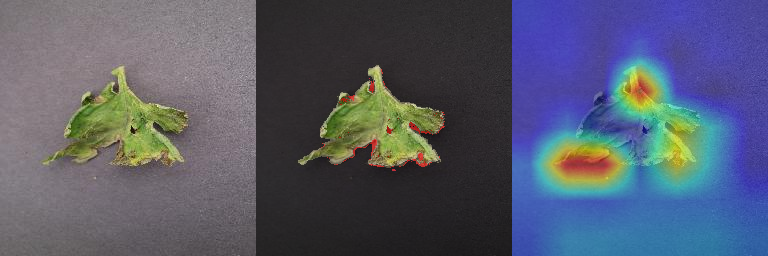
\includegraphics[width=.85\linewidth]{figures/gradcam-severite.png}
\caption{Photo, masque de sévérité (lésions en rouge) et Grad-CAM.}\label{fig:cam}
\end{figure}

\section{Optimisation du modèle}
\subsection{Export ONNX}
Le modèle est exporté en ONNX (opset 17, axe de batch dynamique). La parité avec PyTorch est vérifiée par assertion : écart maximal des logits de $4,9\cdot10^{-5}$, même classe prédite sur toutes les images de contrôle.

\subsection{Quantification INT8 mixte guidée par la sensibilité}
La quantification statique de \emph{toutes} les couches (format QDQ, poids INT8 par canal, activations UINT8, calibration MinMax sur des images d'entraînement) fait tomber l'exactitude à \textbf{4\,\%}. L'analyse montre la cause : le BatchNorm fusionné dans les convolutions laisse, dans les deux premières couches, des canaux aux plages très différentes (écart-type des poids de 0,005 à 6,5). Avec une seule échelle d'activation par tenseur, la plupart des canaux sont écrasés.

Notre solution, automatisée dans \texttt{export.py} :
\begin{enumerate}
  \item chaque couche (Conv ou Gemm) est quantifiée seule, et la dérive moyenne de ses logits par rapport au FP32 est mesurée ;
  \item les couches les plus sensibles sont gardées en FP32, en commençant par la plus sensible, jusqu'à atteindre 98\,\% d'accord avec le FP32.
\end{enumerate}
Résultat : 4 couches sur 54 restent en FP32.
\begin{table}[H]\centering
\begin{tabular}{lcccc}\toprule
Variante & Taille & Latence CPU (1 image) & Exactitude* & Accord avec FP32\\\midrule
PyTorch & 6,4 Mo & 5,72 ms & -- & --\\
ONNX FP32 (servie) & 6,24 Mo & \textbf{1,52 ms} & 99,1\,\% & référence\\
ONNX INT8 mixte & \textbf{1,88 Mo} & 1,90 ms & 98,2\,\% & 97,3\,\%\\
ONNX FP16 & 3,15 Mo & 7,54 ms & 99,1\,\% & 100\,\%\\\bottomrule
\end{tabular}
\caption{Variantes servies par ONNX Runtime (CPU, 4 cœurs). *225 images PlantVillage disjointes de la calibration.}
\end{table}
\textbf{Analyse critique} :
\begin{itemize}
  \item ONNX Runtime divise la latence par 3,8 par rapport à PyTorch.
  \item L'INT8 réduit la taille de 70\,\% mais n'accélère pas ce petit réseau : les nœuds de quantification et de déquantification coûtent autant que le gain des noyaux INT8.
  \item Le FP16 est plus lent sur CPU (pas de noyaux FP16 natifs) ; il est destiné au GPU.
\end{itemize}
Nous servons donc le FP32 par défaut. L'INT8 est disponible via \texttt{ONNX\_VARIANT=int8} pour les déploiements où la mémoire compte (mobile, embarqué).

\section{Cycle de vie MLOps}
\subsection{DVC}
\texttt{dvc.yaml} définit 4 étapes : \texttt{prepare} $\rightarrow$ \texttt{train} $\rightarrow$ \texttt{evaluate} $\rightarrow$ \texttt{export}. Elles dépendent du code, des données et de \texttt{params.yaml}. \texttt{dvc repro} ne relance que les étapes concernées par un changement. Les métriques (\texttt{reports/*.json}) et les courbes sont lisibles avec \texttt{dvc metrics show} et \texttt{dvc plots show}. Les poids (\texttt{.pt}, \texttt{.onnx}) sont des sorties DVC, exclues de Git.

\subsection{MLflow}
Chaque run journalise :
\begin{itemize}
  \item tous les hyperparamètres et le nombre de paramètres du modèle ;
  \item les métriques par epoch (perte, exactitude, F1 macro en entraînement et en validation) et les métriques de test ;
  \item des artefacts : historique, courbes, matrice de confusion, rapport par classe, checkpoint, modèle ONNX et métadonnées de service.
\end{itemize}
Le modèle ONNX est enregistré dans le \textbf{Model Registry} (\texttt{phytora-classifier}) avec l'alias \texttt{staging}. Il est promu en \texttt{production} seulement si son F1 macro de test dépasse celui de la version en production.

\subsection{Conteneurisation et CI/CD}
Chaque service a un Dockerfile multi-stage :
\begin{itemize}
  \item API : environnement virtuel construit à part, image d'exécution réduite avec un utilisateur non root ;
  \item passerelle : dépendances de production uniquement ;
  \item frontend : sortie \emph{standalone} de Next.js.
\end{itemize}
\texttt{docker compose up --build} démarre MongoDB, MLflow, l'API, la passerelle et le frontend, avec des contrôles de santé. Deux workflows GitHub Actions s'exécutent :
\begin{itemize}
  \item \texttt{ci-tests.yml} : flake8 et black, validation de \texttt{dvc.yaml}, 26 tests pytest (pipeline et API), ESLint et 15 tests de la passerelle avec MongoDB en mémoire, ESLint et build du frontend ;
  \item \texttt{docker-build.yml} : build des 3 images, puis test de bout en bout avec \texttt{docker compose up} en mode démonstration (santé, métadonnées, prédiction, code 400 sur un fichier non image).
\end{itemize}

\section{Solution logicielle}
\subsection{API FastAPI}
Les routes \texttt{/health}, \texttt{/model/metadata}, \texttt{/predict}, \texttt{/predict/visualize} et \texttt{/predict/batch} sont asynchrones : l'inférence s'exécute dans un pool de threads. Toutes les entrées et sorties sont validées par des schémas Pydantic stricts (\texttt{extra="forbid"}) et documentées dans Swagger (\texttt{/docs}). Codes d'erreur sémantiques :
\begin{itemize}
  \item 400 : le fichier n'est pas une image ;
  \item 413 : image trop grande ;
  \item 422 : paramètres invalides ;
  \item 501 : explicabilité indisponible ;
  \item 503 : modèle non chargé.
\end{itemize}
Chaque réponse détaille ses latences : prétraitement, inférence et explicabilité.

\subsection{Application web}
\begin{itemize}
  \item \textbf{Ingestion} :
    \begin{itemize}
      \item glisser-déposer, galerie d'exemples, capture webcam ;
      \item \textbf{diagnostic en direct} : une image envoyée toutes les 0,7\,s, une seule requête à la fois, étiquette et barres superposées au flux vidéo, images par seconde affichées.
    \end{itemize}
  \item \textbf{Résultat} : barres de probabilité animées, Grad-CAM, masque de sévérité, latences client, passerelle, serveur et modèle (figure~\ref{fig:ui}).
  \item \textbf{Page Modèle} : métriques, comparaison des architectures, tableau des variantes ONNX, mesure de latence lancée depuis le navigateur.
\end{itemize}
\begin{figure}[H]\centering
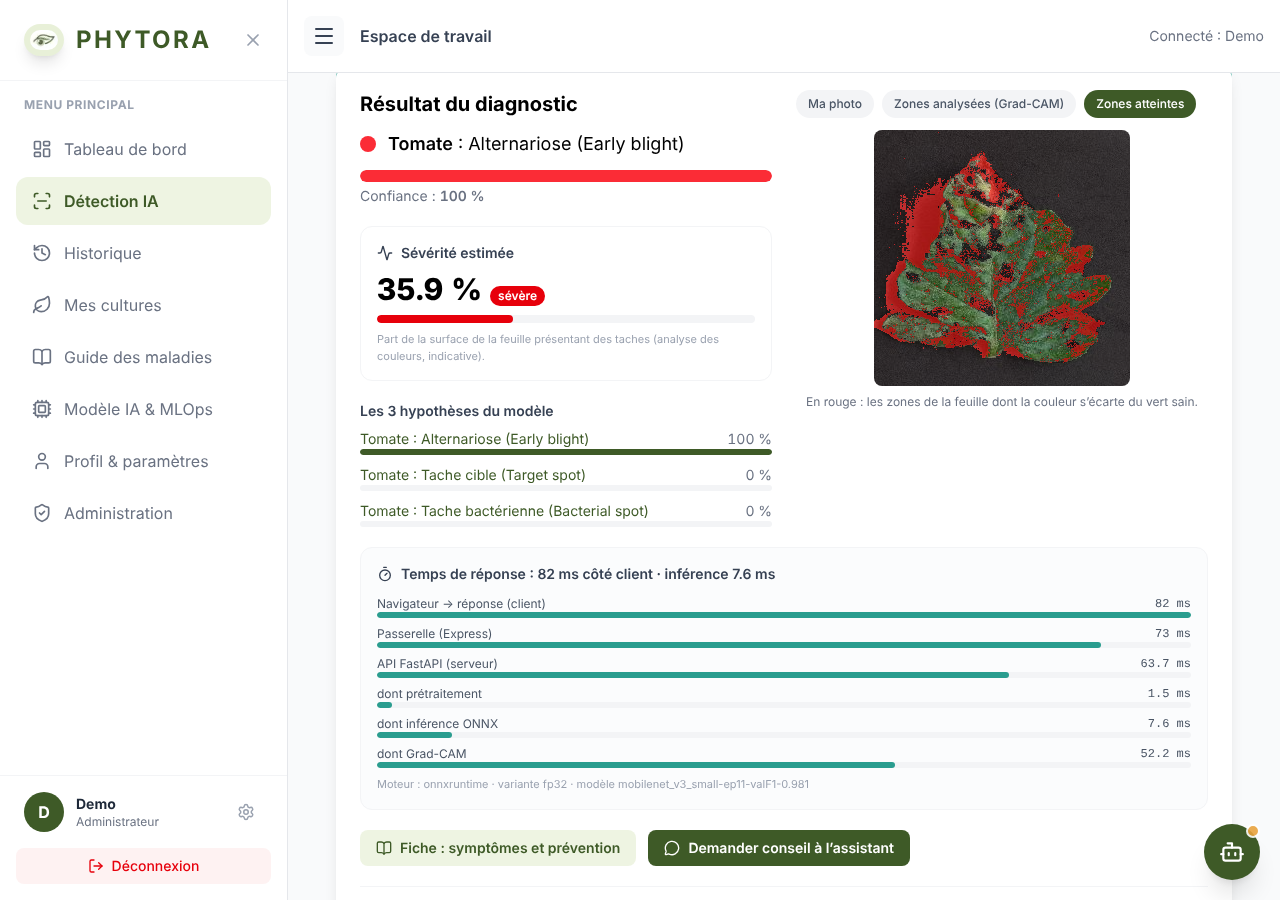
\includegraphics[width=.49\linewidth]{figures/ui-diagnostic.png}\hfill
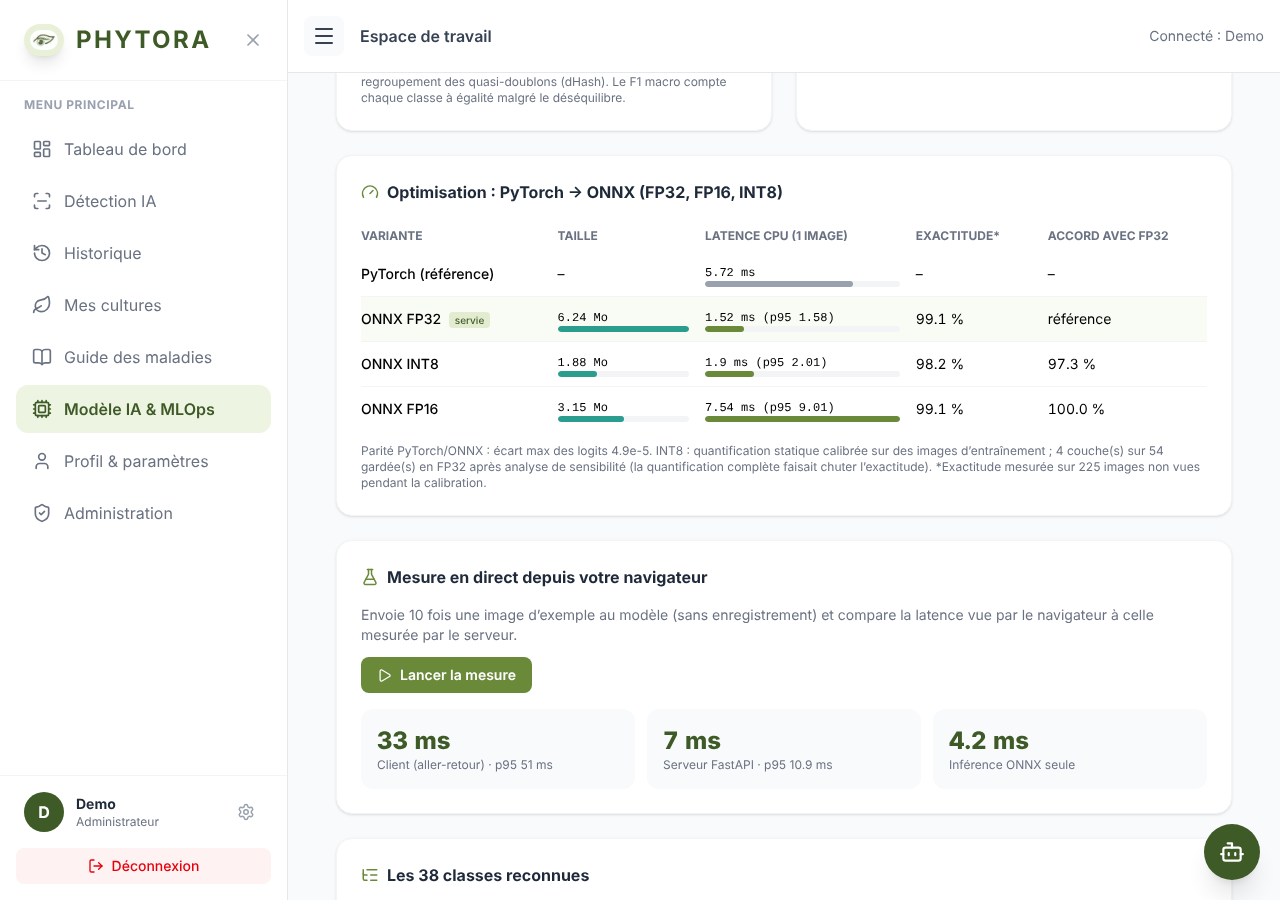
\includegraphics[width=.49\linewidth]{figures/ui-modele.png}
\caption{Résultat d'un diagnostic avec sévérité et latences (gauche) ; page Modèle IA \& MLOps (droite).}\label{fig:ui}
\end{figure}

\subsection{Assistant agronomique (RAG)}
L'assistant (Llama 3.3 70B via Groq) répond au fil de l'eau (Server-Sent Events) avec plusieurs garde-fous :
\begin{itemize}
  \item \textbf{ancrage} : une recherche TF-IDF dans les 38 fiches du guide (avec synonymes français et anglais) sélectionne 3 fiches, injectées et citées [1], [2]\dots ;
  \item \textbf{contexte} : le diagnostic de l'utilisateur et sa sévérité sont relus depuis la base, et un diagnostic appartenant à un autre utilisateur n'est jamais rattaché ;
  \item \textbf{sécurité} : aucun dosage de pesticide, renvoi vers un agronome en cas de doute.
\end{itemize}
Les conversations sont stockées dans MongoDB, et les notes positives et négatives sont résumées dans la page d'administration.
\begin{figure}[H]\centering
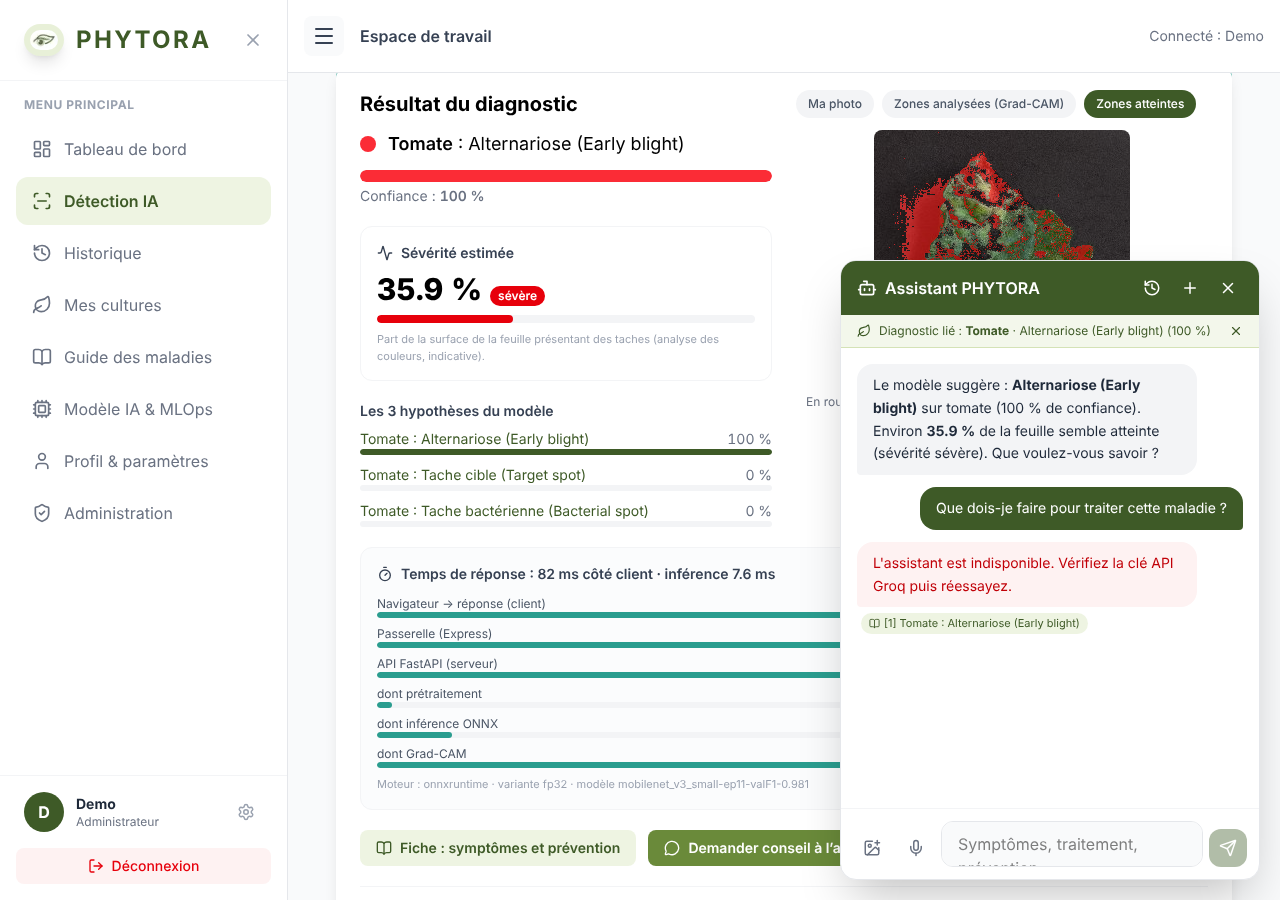
\includegraphics[width=.6\linewidth]{figures/ui-assistant.png}
\caption{Assistant lié au diagnostic, avec la fiche citée.}
\end{figure}

\section{Limites et perspectives}
\begin{itemize}
  \item \textbf{Biais de laboratoire} : les photos de PlantVillage montrent une feuille isolée sur fond uni. Il faut évaluer le modèle sur des photos de terrain (PlantDoc) ; les retours « diagnostic correct ? » collectés constituent un premier jeu de terrain.
  \item \textbf{Score optimiste} : le dHash ne regroupe pas les différentes photos d'une même feuille.
  \item \textbf{Calibration} : les seuils d'incertitude (confiance $<0,6$ ou marge $<0,1$) sont à calibrer, par exemple par \emph{temperature scaling}.
  \item \textbf{Perspectives} :
    \begin{itemize}
      \item segmentation des lésions apprise (U-Net) pour remplacer l'heuristique de sévérité ;
      \item entraînement sensible à la quantification (QAT) pour un INT8 complet ;
      \item suivi de la dérive en production (Prometheus et Grafana).
    \end{itemize}
\end{itemize}

\section*{Reproduire}
\begin{lstlisting}
dvc pull && cp .env.example .env && docker compose up --build
# entrainement : pip install -r requirements-train.txt && dvc repro
\end{lstlisting}
\end{document}
